% =====================================================================
%  CSE499A — AI Medical Pre-Screening Assistant
%  Chapter: Project Design (Updated) — ≤10 pages
%  Authors: Rafiur Rahman Mashrafi (2221971042),
%           M.G. Rabbi Hossen (2222516042),
%           Israt Zaman Srity (2211084042)
%  Advisor: Dr. Mohammad Ashrafuzzaman Khan [AzK]
%  Dept. of ECE, North South University · Spring 2026
% =====================================================================
\documentclass[11pt,a4paper]{article}

\usepackage[utf8]{inputenc}
\usepackage[T1]{fontenc}
\usepackage{mathptmx}
\usepackage[a4paper, top=0.85in, bottom=0.85in, left=0.9in, right=0.9in]{geometry}
\usepackage{setspace}
\usepackage{enumitem}
\usepackage{booktabs}
\usepackage{tabularx}
\usepackage{array}
\usepackage{multicol}
\usepackage{tikz}
\usepackage[hidelinks]{hyperref}
\usepackage{titlesec}
\usepackage{xcolor}
\usepackage{caption}
\usepackage{float}
\usepackage{parskip}

\usetikzlibrary{shapes,shapes.geometric,arrows.meta,positioning,fit,backgrounds,shadows,calc}
\usepackage{wasysym}

\setstretch{1.1}
\setlength{\parskip}{3pt}
\setlength{\parindent}{0pt}

\titleformat{\section}{\normalfont\large\bfseries}{\thesection}{0.6em}{}[\vspace{-4pt}\rule{\linewidth}{0.4pt}]
\titleformat{\subsection}{\normalfont\normalsize\bfseries}{\thesubsection}{0.5em}{}
\titlespacing{\section}{0pt}{8pt}{4pt}
\titlespacing{\subsection}{0pt}{5pt}{2pt}

% ── colour palette ──────────────────────────────────────────────────
\definecolor{modblue}{RGB}{52,101,164}
\definecolor{modbluelt}{RGB}{210,225,245}
\definecolor{alertred}{RGB}{192,0,0}
\definecolor{alertlt}{RGB}{255,220,220}
\definecolor{looporg}{RGB}{180,95,6}
\definecolor{looporlt}{RGB}{255,235,205}
\definecolor{dbgray}{RGB}{80,80,80}
\definecolor{dbgraylt}{RGB}{230,230,230}
\definecolor{greenlt}{RGB}{200,235,200}
\definecolor{greendark}{RGB}{30,120,30}
\definecolor{headgray}{RGB}{50,50,50}

\captionsetup{font=small,labelfont=bf,skip=4pt}

% ── TikZ styles ─────────────────────────────────────────────────────
\tikzset{
  mod/.style={rectangle, rounded corners=4pt,
    draw=modblue, fill=modbluelt, line width=0.8pt,
    text width=28mm, minimum height=9mm, align=center,
    font=\scriptsize\bfseries\color{modblue}, drop shadow},
  alertmod/.style={rectangle, rounded corners=4pt,
    draw=alertred, fill=alertlt, line width=1pt,
    text width=28mm, minimum height=9mm, align=center,
    font=\scriptsize\bfseries\color{alertred}, drop shadow},
  loopmod/.style={rectangle, rounded corners=4pt,
    draw=looporg, fill=looporlt, line width=0.8pt,
    text width=28mm, minimum height=9mm, align=center,
    font=\scriptsize\bfseries\color{looporg}, drop shadow},
  dbmod/.style={cylinder, draw=dbgray, fill=dbgraylt,
    shape border rotate=90, aspect=0.3,
    text width=22mm, minimum height=9mm, align=center,
    font=\scriptsize\bfseries\color{dbgray}, drop shadow},
  greenmod/.style={rectangle, rounded corners=4pt,
    draw=greendark, fill=greenlt, line width=0.8pt,
    text width=28mm, minimum height=9mm, align=center,
    font=\scriptsize\bfseries\color{greendark}, drop shadow},
  decision/.style={diamond, draw=looporg, fill=looporlt,
    line width=0.8pt, aspect=2.2,
    text width=20mm, minimum height=8mm, align=center,
    font=\tiny\bfseries\color{looporg}, drop shadow},
  arr/.style={-{Stealth[length=4pt]}, line width=0.7pt, color=headgray},
  redarr/.style={-{Stealth[length=4pt]}, line width=0.9pt, color=alertred},
  orgarr/.style={-{Stealth[length=4pt]}, line width=0.7pt, color=looporg},
  grnarr/.style={-{Stealth[length=4pt]}, line width=0.7pt, color=greendark},
  lbl/.style={font=\tiny, color=headgray}
}

% ====================================================================
\title{\vspace{-18pt}\bfseries\large Project Design (Updated)\\[3pt]
{\normalsize AI Medical Pre-Screening Assistant}\\
{\small EHR-Based Pre-Consultation Medical Documentation System}}
\author{\small Rafiur Rahman Mashrafi (2221971042)\quad
        M.~G.~Rabbi Hossen (2222516042)\quad
        Israt Zaman Srity (2211084042)\\[3pt]
        \small\emph{Advisor:} Dr.~Mohammad Ashrafuzzaman Khan [AzK]\\
        \small Dept.\ of ECE, North South University, Bangladesh}
\date{\small CSE499A — Spring 2026}

\begin{document}
\maketitle\vspace{-10pt}
\rule{\linewidth}{0.6pt}

% ====================================================================
\section{Introduction}
% ====================================================================

This chapter presents the \textbf{updated} design of the \textit{AI
Medical Pre-Screening Assistant}. The original CSE499A design was a
five-stage, one-shot pipeline: patient speech $\to$ ASR $\to$ Medical
NER $\to$ Structured EHR $\to$ Doctor Dashboard. Based on empirical
findings from Phases~2 and~3 and a review of clinical NLP requirements,
the design has been expanded to \textbf{15 functional modules} that add:
an adaptive conversational follow-up loop, emergency detection,
risk classification, explainable AI, and a continuous feedback and
learning mechanism. The system remains a \textit{pre-screening and
decision-support tool}; all final clinical decisions belong to the
attending physician.

% ====================================================================
\section{Design Comparison: Original vs.\ Updated}
% ====================================================================

\begin{center}
\footnotesize
\setlength{\tabcolsep}{4pt}
\renewcommand{\arraystretch}{1.25}
\begin{tabularx}{\linewidth}{>{\bfseries}p{2.8cm} X X}
\toprule
Dimension & \textbf{Original (5 stages)} & \textbf{Updated (15 modules)} \\
\midrule
Interaction model   & One-shot recording; no follow-up
                    & Conversational loop; adaptive follow-up until profile is complete \\
Emergency detection & Absent
                    & Module~5: rule-based + AI classifier; immediate alert pathway \\
Information gaps    & Absent
                    & Module~6: structured completeness checklist per symptom category \\
Risk classification & Differential hints only
                    & Module~10: Low / Medium / High / Critical with clinical rule engine \\
Explainability      & Absent
                    & Module~11 (XAI): plain-language driver explanations for every risk score \\
Clinical report     & Basic structured EHR
                    & Module~12: full 8-section pre-screening report; PDF + dashboard export \\
Feedback \& learning & Absent
                    & Module~15: doctor annotations feed model retraining pipeline \\
Bangla support      & ASR \& transcript only
                    & End-to-end bilingual; follow-up questions generated in Bangla or English \\
\bottomrule
\end{tabularx}
\end{center}

% ====================================================================
\section{Updated System Architecture — 15 Modules}
% ====================================================================

\subsection{Complete Pipeline Diagram}

\begin{figure}[H]
\centering
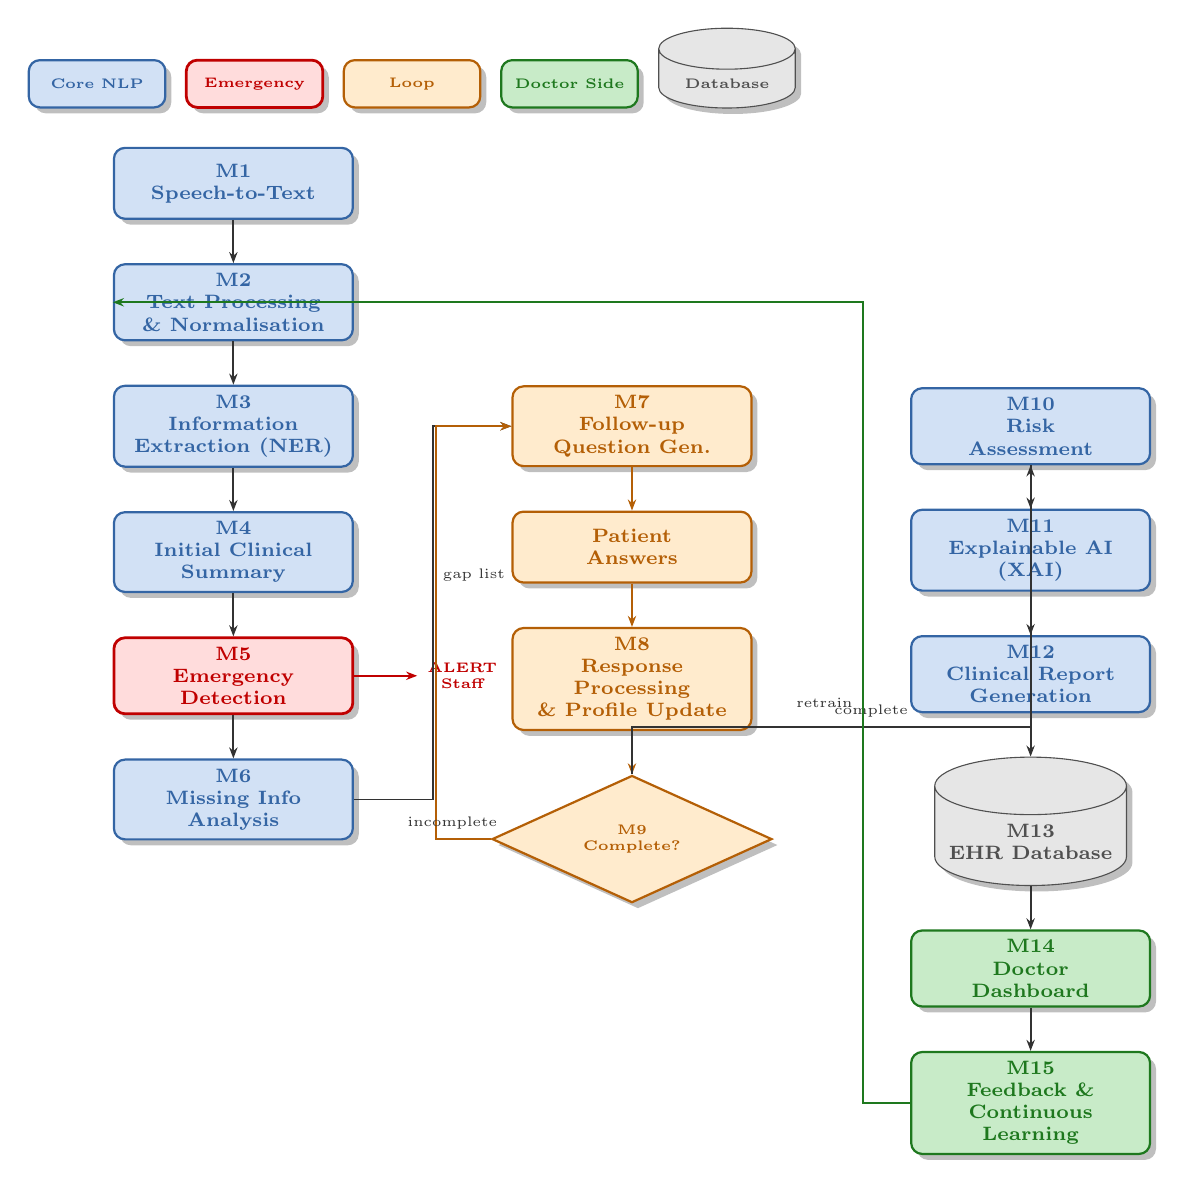
\begin{tikzpicture}[node distance=5.5mm and 6mm]

%% ── COLUMN A: Core NLP (left) ──────────────────────────────────────
\node[mod]      (m1)  {M1\\Speech-to-Text};
\node[mod, below=of m1] (m2)  {M2\\Text Processing\\\& Normalisation};
\node[mod, below=of m2] (m3)  {M3\\Information\\Extraction (NER)};
\node[mod, below=of m3] (m4)  {M4\\Initial Clinical\\Summary};
\node[alertmod, below=of m4] (m5)  {M5\\Emergency\\Detection};
\node[mod, below=of m5] (m6)  {M6\\Missing Info\\Analysis};

%% ── COLUMN B: Loop (centre) ────────────────────────────────────────
\node[loopmod, right=20mm of m3] (m7) {M7\\Follow-up\\Question Gen.};
\node[loopmod, below=of m7]      (pat){Patient\\Answers};
\node[loopmod, below=of pat]     (m8) {M8\\Response Processing\\\& Profile Update};
\node[decision, below=of m8]     (m9) {M9\\Complete?};

%% ── COLUMN C: Assessment + Storage (right) ──────────────────────────
\node[mod,      right=20mm of m7]  (m10){M10\\Risk\\Assessment};
\node[mod,      below=of m10]      (m11){M11\\Explainable AI\\(XAI)};
\node[mod,      below=of m11]      (m12){M12\\Clinical Report\\Generation};
\node[dbmod,    below=of m12]      (m13){M13\\EHR Database};
\node[greenmod, below=of m13]      (m14){M14\\Doctor\\Dashboard};
\node[greenmod, below=of m14]      (m15){M15\\Feedback \&\\Continuous Learning};

%% ── ARROWS: Column A ───────────────────────────────────────────────
\draw[arr] (m1)--(m2);
\draw[arr] (m2)--(m3);
\draw[arr] (m3)--(m4);
\draw[arr] (m4)--(m5);
\draw[arr] (m5)--(m6);

%% Emergency side exit
\draw[redarr] (m5.east) --++(8mm,0)
  node[right, align=center, font=\tiny\bfseries\color{alertred}]{ALERT\\Staff};

%% M6 → M7
\draw[arr] (m6.east) -| ($(m6.east)+(10mm,0)$) |-
  node[lbl, pos=0.3, right]{gap list} (m7.west);

%% ── ARROWS: Loop ───────────────────────────────────────────────────
\draw[orgarr] (m7)--(pat);
\draw[orgarr] (pat)--(m8);
\draw[orgarr] (m8)--(m9);

%% M9 → incomplete back to M7
\draw[orgarr] (m9.west) --++(-7mm,0)
  node[lbl, above, pos=0.7]{incomplete}
  |- ($(m7.west)+(-7mm,0)$) -- (m7.west);

%% M9 → complete → M10
\draw[arr] (m9.north) -- ($(m9.north)+(0,6mm)$)
  -| node[lbl, pos=0.3, above]{complete} (m10.south);

%% ── ARROWS: Column C ───────────────────────────────────────────────
\draw[arr] (m10)--(m11);
\draw[arr] (m11)--(m12);
\draw[arr] (m12)--(m13);
\draw[arr] (m13)--(m14);
\draw[arr] (m14)--(m15);

%% Feedback loop back
\draw[grnarr] (m15.west) --++(-6mm,0)
  |- node[lbl, pos=0.25, left]{retrain} (m2.west);

%% ── LEGEND box ─────────────────────────────────────────────────────
\begin{scope}[shift={($(m1.north west)+(-2mm,8mm)$)}]
  \node[mod,    text width=15mm, minimum height=6mm, font=\tiny\bfseries\color{modblue}]
       at (0,0)   (l1){Core NLP};
  \node[alertmod,text width=15mm, minimum height=6mm, font=\tiny\bfseries\color{alertred}]
       at (20mm,0)(l2){Emergency};
  \node[loopmod, text width=15mm, minimum height=6mm, font=\tiny\bfseries\color{looporg}]
       at (40mm,0)(l3){Loop};
  \node[greenmod,text width=15mm, minimum height=6mm, font=\tiny\bfseries\color{greendark}]
       at (60mm,0)(l4){Doctor Side};
  \node[dbmod,   text width=15mm, minimum height=6mm, font=\tiny\bfseries\color{dbgray}]
       at (80mm,0)(l5){Database};
\end{scope}

\end{tikzpicture}
\caption{Complete 15-module pipeline. Orange = adaptive follow-up loop;
         red = emergency escalation path; green = doctor-facing modules.}
\label{fig:pipeline}
\end{figure}

\subsection{Module Descriptions}

\begin{description}[leftmargin=0pt, labelwidth=0pt, style=nextline,
                    itemsep=2pt, parsep=0pt]

\item[\textbf{M1 — Speech-to-Text.}]
Accepts Bangla, Banglish, and regional dialect speech. Audio is
VAD-segmented into 10--15\,s clips and transcribed by the
best-performing ASR model identified in Phase~2
(\textit{BengaliAI Regional}: 46.94\% WER on dialect; target for
CSE499B fine-tuning: $<$20\% WER via LoRA on Qwen3-ASR-1.7B).

\item[\textbf{M2 — Text Processing \& Normalisation.}]
Spelling correction, Banglish normalisation, filler removal, punctuation
restoration, and sentence-boundary detection. Bilingual
Bangla--English handling throughout.

\item[\textbf{M3 — Information Extraction (NER).}]
BanglaBERT token classifier labels: \textit{symptom, affected site,
duration, severity, frequency, age, comorbidity, medication}. Temporal
expressions normalised to ISO~8601-like intervals.

\item[\textbf{M4 — Initial Clinical Summary.}]
Short human-readable summary of the chief complaint, e.g.\ \textit{``Fever
and dry cough for 3 days; mild fatigue; no dyspnoea or chest pain.''}
Used downstream and displayed on the dashboard.

\item[\textbf{M5 — Emergency Detection} \textcolor{alertred}{(new).}]
Rule-based critical-symptom checker + AI classifier for ambiguous
presentations. Red-flag triggers: chest pain, stroke indicators, severe
dyspnoea, loss of consciousness, acute trauma. Escalates immediately;
bypasses the normal pipeline flow.

\item[\textbf{M6 — Missing Information Analysis} \textcolor{alertred}{(new).}]
Compares extracted entities against a per-symptom clinical checklist and
outputs a structured gap report (e.g.\ \CheckedBox~Fever detected;
\XBox~Duration not specified; \XBox~Temperature not provided).

\item[\textbf{M7 — Follow-up Question Generation} \textcolor{looporg}{(new).}]
Generates clinically prioritised questions in Bangla or English to fill
identified gaps. Avoids repeating answered items. Example:
\textit{``Apnar jwor ki matro kal theke?''} / \textit{``When did the fever start?''}

\item[\textbf{M8 — Response Processing \& Profile Update} \textcolor{looporg}{(new).}]
Patient answers re-enter Modules~2--3. Extracted entities are merged into
the profile with conflict resolution; filled gaps are marked.

\item[\textbf{M9 — Case Completion Check} \textcolor{looporg}{(new).}]
Scores profile completeness against a configurable threshold.
If incomplete: loops back to M7. If complete (or max turns reached):
continues to M10.

\item[\textbf{M10 — Risk Assessment} \textcolor{alertred}{(new).}]
Assigns one of four tiers — \textbf{Low / Medium / High / Critical} —
using a clinical rule engine weighted by age, comorbidities, severity,
and duration. Integrates M5 output.

\item[\textbf{M11 — Explainable AI (XAI)} \textcolor{alertred}{(new).}]
SHAP/LIME feature attribution converted to plain language: e.g.\
\textit{``High risk: fever $>$5 days + dyspnoea + age $>$65.''}
Displayed alongside every risk classification.

\item[\textbf{M12 — Clinical Report Generation} \textcolor{alertred}{(new).}]
Produces an 8-section pre-screening report: Patient Profile, Chief
Complaint, Symptoms, Emergency Flags, Q\&A Log, Risk Level + XAI,
Possible Condition Categories, Recommended Next Steps. Exported as PDF
and to the dashboard.

\item[\textbf{M13 — EHR Database.}]
HIPAA/PDPA-compliant PostgreSQL store with encryption at rest and in
transit. Stores transcripts, extracted data, follow-up exchanges, risk
assessments, and final reports. Full audit logging.

\item[\textbf{M14 — Doctor Dashboard} (extended from original).]
Displays the report, risk tier, emergency flags, and XAI explanation.
Supports annotation and override of any extracted field (all changes
versioned). Real-time notifications for High/Critical cases.

\item[\textbf{M15 — Feedback \& Continuous Learning} \textcolor{greendark}{(new).}]
Doctors rate reports, correct extractions, flag missed symptoms, and
annotate risk disagreements. Feedback drives periodic model retraining
for M3, M7, and M10, subject to regression testing before deployment.

\end{description}

% ====================================================================
\section{System Flowchart — Patient Journey}
% ====================================================================

\begin{figure}[H]
\centering
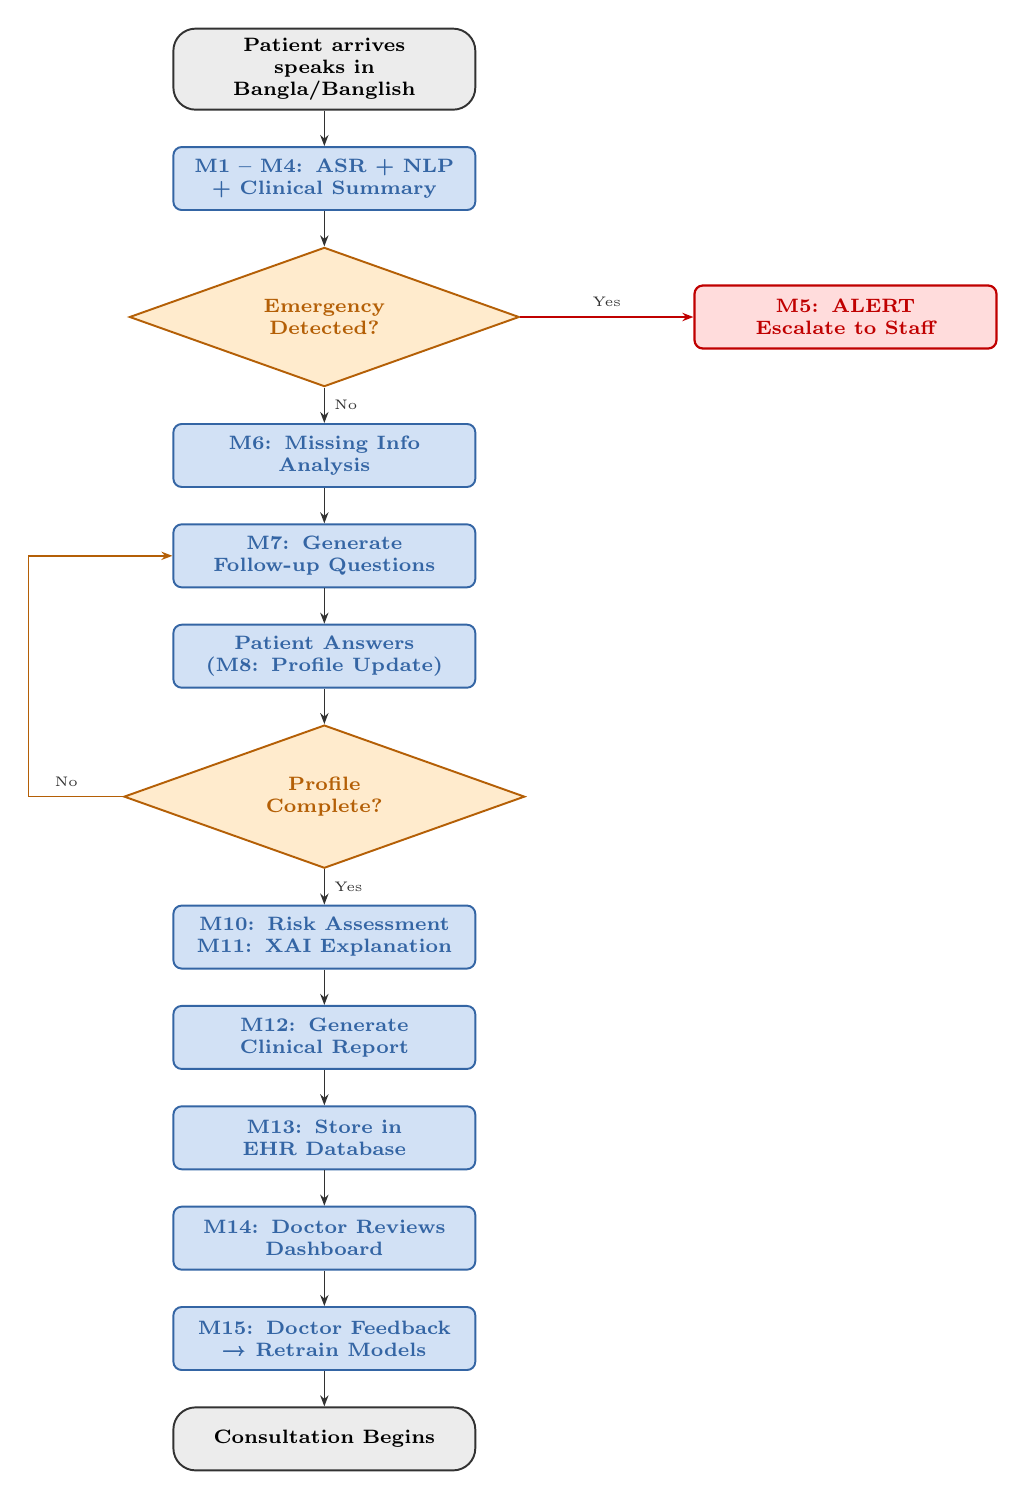
\begin{tikzpicture}[node distance=4.5mm and 10mm,
  proc/.style={rectangle, rounded corners=3pt,
    draw=modblue, fill=modbluelt, line width=0.7pt,
    text width=36mm, minimum height=8mm, align=center,
    font=\scriptsize\bfseries\color{modblue}},
  term/.style={rectangle, rounded corners=8pt,
    draw=headgray, fill=gray!15, line width=0.7pt,
    text width=36mm, minimum height=8mm, align=center,
    font=\scriptsize\bfseries},
  dec/.style={diamond, draw=looporg, fill=looporlt,
    line width=0.7pt, aspect=2.8,
    text width=28mm, minimum height=7mm, align=center,
    font=\scriptsize\bfseries\color{looporg}},
  alrt/.style={rectangle, rounded corners=3pt,
    draw=alertred, fill=alertlt, line width=0.8pt,
    text width=36mm, minimum height=8mm, align=center,
    font=\scriptsize\bfseries\color{alertred}},
  arr/.style={-{Stealth[length=4pt]}, line width=0.6pt, color=headgray},
  redarr/.style={-{Stealth[length=4pt]}, line width=0.8pt, color=alertred},
  orgarr/.style={-{Stealth[length=4pt]}, line width=0.6pt, color=looporg},
  lbl/.style={font=\tiny, color=headgray}
]

\node[term]  (start) {Patient arrives\\speaks in Bangla/Banglish};
\node[proc, below=of start]  (asr)   {M1 -- M4: ASR + NLP\\+ Clinical Summary};
\node[dec,  below=of asr]    (emerg) {Emergency\\Detected?};
\node[alrt, right=22mm of emerg] (alert){M5: ALERT\\Escalate to Staff};
\node[proc, below=of emerg]  (gap)   {M6: Missing Info\\Analysis};
\node[proc, below=of gap]    (qgen)  {M7: Generate\\Follow-up Questions};
\node[proc, below=of qgen]   (pans)  {Patient Answers\\(M8: Profile Update)};
\node[dec,  below=of pans]   (comp)  {Profile\\Complete?};
\node[proc, below=of comp]   (risk)  {M10: Risk Assessment\\M11: XAI Explanation};
\node[proc, below=of risk]   (rep)   {M12: Generate\\Clinical Report};
\node[proc, below=of rep]    (store) {M13: Store in\\EHR Database};
\node[proc, below=of store]  (dash)  {M14: Doctor Reviews\\Dashboard};
\node[proc, below=of dash]   (fb)    {M15: Doctor Feedback\\→ Retrain Models};
\node[term, below=of fb]     (end)   {Consultation Begins};

%% Main flow
\draw[arr] (start)--(asr);
\draw[arr] (asr)--(emerg);
\draw[redarr] (emerg.east)--node[lbl,above]{Yes}(alert.west);
\draw[arr] (emerg.south)--node[lbl,right]{No}(gap);
\draw[arr] (gap)--(qgen);
\draw[arr] (qgen)--(pans);
\draw[arr] (pans)--(comp);
%% Loop back
\draw[orgarr] (comp.west)--++(-12mm,0)
  node[lbl,above,pos=0.6]{No}
  |-($(qgen.west)+(-12mm,0)$)--(qgen.west);
\draw[arr] (comp.south)--node[lbl,right]{Yes}(risk);
\draw[arr] (risk)--(rep);
\draw[arr] (rep)--(store);
\draw[arr] (store)--(dash);
\draw[arr] (dash)--(fb);
\draw[arr] (fb)--(end);

\end{tikzpicture}
\caption{Patient journey flowchart through all 15 modules.
         The orange loop iterates until the clinical profile is sufficiently complete.}
\label{fig:flowchart}
\end{figure}

% ====================================================================
\section{Software Components}
% ====================================================================

\footnotesize\setlength{\tabcolsep}{3pt}\renewcommand{\arraystretch}{1.2}
\begin{tabularx}{\linewidth}{>{\bfseries}p{2.4cm} p{3.2cm} X}
\toprule
Tool & Function & Rationale \\
\midrule
Python 3.10        & Implementation language           & Standard ML/NLP ecosystem \\
PyTorch 2.x        & Deep-learning framework           & Native support across all benchmarked ASR models \\
HF Transformers    & Model loading \& inference        & Unified API: Whisper, Wav2Vec2, MMS, Qwen-Audio, Phi-4 \\
HF PEFT / Accelerate & LoRA fine-tuning (CSE499B)     & Lowest friction with Transformers for parameter-efficient tuning \\
BanglaBERT         & Medical NER (M3)                  & Pre-trained on large Bangla corpus; best Bangla NLP results \\
WhisperX           & VAD segmentation (M1)             & Required for audio $>$30\,s; forced alignment \\
LIME / SHAP        & XAI feature attribution (M11)     & Standard, well-documented explainability libraries \\
FastAPI            & Backend REST/WebSocket (M8--M13)  & Async; low latency for real-time follow-up dialogue \\
PostgreSQL         & EHR database (M13)                & Mature; encryption-at-rest support; HIPAA-ready \\
React / Next.js    & Doctor dashboard (M14)            & Low-bandwidth responsive UI; role-based access \\
Flutter / PWA      & Patient kiosk app (M1 interface)  & Low-tech-literacy UX; single record button; Bangla prompts \\
MLflow             & Feedback \& retraining (M15)      & Experiment tracking; model versioning \\
\texttt{jiwer}     & WER / CER / BLEU scoring          & Standard ASR evaluation metric library \\
Google Colab       & GPU compute (T4 / A100)           & Free tier sufficient for inference benchmarks \\
\bottomrule
\end{tabularx}
\normalsize

% ====================================================================
\section{CSE499A Implementation Phases}
% ====================================================================

\begin{description}[leftmargin=0pt, style=nextline, itemsep=2pt, parsep=0pt]

\item[\textbf{Phase 1 — Audio Collection \& Preprocessing}] \textit{Demo: 12 Mar 2026.}
Multi-dialect corpus assembled (Dhakaiya, Barishali, Sylheti, Normal,
Indian Bangla). Files logged in \texttt{dataset\_log.csv}. Preprocessed
to 16\,kHz mono PCM; segmented by WhisperX VAD.
Final corpus: $\approx$4.7\,h, 10 sources, $\sim$1{,}100 clips.

\item[\textbf{Phase 2 — Baseline ASR Benchmark (12 models)}] \textit{Demo: 2 Apr 2026.}
Whisper (S/M/L/Turbo), Wav2Vec2 variants, MMS, Vakyansh-Bn, BengaliAI
Whisper/Regional, SeamlessM4T. Best: \textbf{BengaliAI Regional}
(46.94\% WER, 24.29\% CER, 0.273 BLEU). Finding: dialect speech
defeats even the best open Bangla models.

\item[\textbf{Phase 3 — Large Multimodal LLM Benchmark}] \textit{Demo: 9 Apr 2026.}
Qwen2-Audio, Qwen3-ASR-1.7B, Voxtral-Mini, Phi-4 Multimodal,
Qwen2.5-Omni (1.7B--7B). None matched BengaliAI Regional;
closest trailed by $>$50 pp WER. Conclusion: \textit{specialisation
beats scale for Bangla dialect ASR}.

\item[\textbf{Phase 4 — Fine-Tuning Research (in progress)}] \textit{Demo: 16 Apr 2026.}
LoRA fine-tuning methodology for Qwen3-ASR-1.7B on the dialect corpus.
Adapter on speech encoder only; decoder frozen. No training run yet —
this is a methodology study for execution in CSE499B.

\item[\textbf{Phase 5 — Chatbot Output Study (selected)}] \textit{Execution: next demo.}
ChatGPT, DeepSeek, Qwen, Perplexity prompted with simulated patient
utterances. Outputs compared on schema consistency, field completeness,
code-mixed handling, and source faithfulness. Result will inform
Module~12 report schema.

\end{description}

% ====================================================================
\section{Conclusion}
% ====================================================================

The updated design addresses the three main limitations of the original
five-stage pipeline: (i)~the adaptive follow-up loop (M6--M9) ensures
clinical information completeness; (ii)~Module~5 provides an explicit
emergency escalation pathway absent from the original design; and
(iii)~Modules~10--11 and~15 add risk stratification, explainability, and
continuous improvement. The empirical finding from Phases~2 and~3 ---
that specialisation beats scale for Bangla dialect ASR --- directly
motivates the CSE499B priority: LoRA fine-tuning of Qwen3-ASR-1.7B.
Once ASR reliability is demonstrated, the application layer (Modules
3--15) will be built iteratively.

% ====================================================================
\begin{thebibliography}{99}\small
\bibitem{w} A.~Radford \emph{et al.}, ``Robust Speech Recognition via Large-Scale Weak Supervision,'' \emph{ICML 2023}. \url{https://arxiv.org/abs/2212.04356}
\bibitem{b} A.~Baevski \emph{et al.}, ``wav2vec 2.0,'' \emph{NeurIPS 2020}.
\bibitem{q} Y.~Chu \emph{et al.}, ``Qwen2-Audio Technical Report,'' \emph{arXiv:2407.10759}, 2024.
\bibitem{t} T.~Wolf \emph{et al.}, ``Transformers,'' \emph{EMNLP 2020}. \url{https://github.com/huggingface/transformers}
\bibitem{l} E.~J.~Hu \emph{et al.}, ``LoRA,'' \emph{ICLR 2022}. \url{https://arxiv.org/abs/2106.09685}
\bibitem{wx} M.~Bain \emph{et al.}, ``WhisperX,'' \emph{INTERSPEECH 2023}. \url{https://arxiv.org/abs/2303.00747}
\bibitem{bb} A.~Bhattacharjee \emph{et al.}, ``BanglaBERT,'' \emph{NAACL 2022 Findings}. \url{https://github.com/csebuetnlp/banglabert}
\bibitem{sh} S.~Lundberg \& S.~Lee, ``SHAP,'' \emph{NeurIPS 2017}. \url{https://arxiv.org/abs/1705.07874}
\bibitem{li} M.~Ribeiro \emph{et al.}, ``LIME,'' \emph{KDD 2016}. \url{https://arxiv.org/abs/1602.04938}
\bibitem{oo} F.~R.~Rakib \emph{et al.}, ``OOD-Speech,'' \emph{INTERSPEECH 2023}. \url{https://arxiv.org/abs/2305.09688}
\end{thebibliography}

\end{document}
